\documentclass{exam}

%%%%%%%%%%%%%%%%%% PACKAGES %%%%%%%%%%%%%%%%%%%%%%%%

\usepackage{amsmath}
\usepackage{amsfonts}
\usepackage{tcolorbox}
\usepackage{tikz,tkz-euclide,tikz-3dplot}

%%%%%%%%%%%%%%%%%% HEADER AND FOOTER %%%%%%%%%%%%%%%

\pagestyle{headandfoot}
\firstpageheadrule
\runningheadrule
\firstpageheader{AP BC Calculus}{}{Mr. Carey}
\runningheader{AP BC Calculus}{}{Mr. Carey}
\firstpagefooter{}{}{}
\runningfooter{ }{\thepage}{ }

%%%%%%%%%%%%%%%%%%%%%%%%%%%%%%%%%%%%%%%%%%%%%%%%%%%%

\begin{document}
\section*{Lagrange Error Bound} 

\begin{tcolorbox}[title=Recall: \textit{Lagrange Error Bound},title filled,colframe=black,sharpish corners,width=\linewidth]
    \[\text{Error}=\left|f(x)-P_n(x)\right|\le\frac{|x-c|^{n+1}}{(n+1)!}\max\left[f^{(n+1)}(z)\right]\text{ where }z\text{ is between }x\text{ and }c.\]
\end{tcolorbox}

\begin{questions} 
    \question The degree 4 Taylor Polynomial for $f(x)$ centered about $x=2$ is given by:
    \[P_4=9+\frac{1}{7}(x-2)^3+7(x-2)^4 .\]
    Using infromation from the graph of $y=f^{(5)}(x)$ below and the Lagrange error bound, approximate the maximum value of $\left|P_4(1.5)-f(1.5)\right|$.

    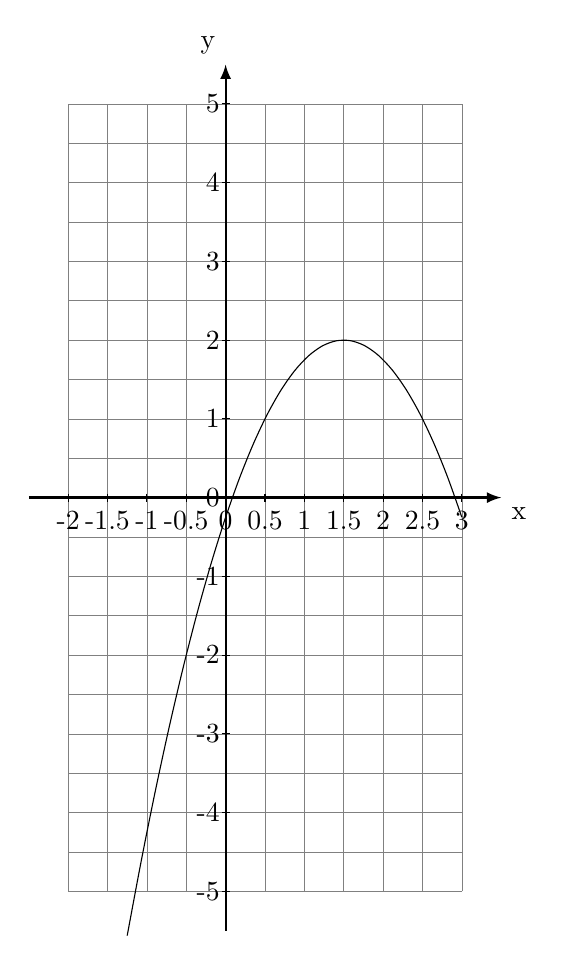
\begin{tikzpicture}
        \draw[step=0.5,gray,very thin] (-2,-5) grid (3,5);
        \foreach
        \x in {-2,-1.5,...,3} {\draw (\x,0.05) -- (\x,-0.05) node[below] {\x};}
        \foreach
        \y in {-5,-4,...,5} {\draw (-0.05,\y) -- (0.05,\y) node[left] {\y};}
        \draw[thick,-latex] (-2.5,0) -- (3.5,0) node[anchor=north west] {x};
        \draw[thick,-latex] (0,-5.5) -- (0,5.5) node[anchor=south east] {y};
        \draw[scale=1, domain=-1.25:3, smooth, variable=\x] plot ({\x}, {-1*(\x-1.5)^2+2});
    \end{tikzpicture}

    \vspace{\stretch{1}}

    \question Consider the Taylor Polynomial for $f$ given by $P_3(x)=-9+\frac{3}{7}(x-3)^2-\frac{1}{9}(x-3)^3$. The fourth derivative of $f(x)$ satisfies the inequality $\displaystyle\left|f^{(4)}(x)\right|\le85$ for all $x\in[3,3.3]$. Find an upper bound for the approximation of $\displaystyle\left|f(3.3)-P_3(3.3)\right|$.
    
    \vspace{\stretch{1}}

   
    
\end{questions}



\end{document}
